\documentclass[a4paper,12pt,fleqn,oneside]{article} 	% Openright aabner kapitler paa hoejresider (openany begge)
\usepackage{svg}
\documentclass[a4paper,12pt,fleqn,oneside]{article} 	% Openright aabner kapitler paa hoejresider (openany begge)

%===== Projekt konstanter =====
\newcommand{\kursusTitel}{Semesterprojekt 3}
\newcommand{\linje}{E/IKT}
\newcommand{\semester}{3}
\newcommand{\system}{Beer Pong Master\copyright}
\newcommand{\rapportType}{Proces}
\newcommand{\gruppeNr}{7}
\newcommand{\vejleder}{Martin Ansbjerg Kjær}
\newcommand{\afleveringsdato}{6/6-2018}

%%%% PAKKER %%%%
% ¤¤ Oversaettelse og tegnsaetning ¤¤ %
\usepackage[utf8]{inputenc}					% Input-indkodning af tegnsaet (UTF8)
\usepackage[english, danish]{babel}					% Dokumentets sprog
\usepackage[T1]{fontenc}					% Output-indkodning af tegnsaet (T1)
\usepackage{ragged2e,anyfontsize}			% Justering af elementer

% ¤¤ Figurer og tabeller (floats) ¤¤ %
\usepackage{wrapfig} % text wrapping
\usepackage{graphicx} 						% Haandtering af eksterne billeder (JPG, PNG, PDF)
\usepackage{caption}
\usepackage{subcaption}
\usepackage{multirow}                		% Fletning af raekker og kolonner (\multicolumn og \multirow)
\usepackage{makecell}                       % Line breaks i tabelceller med \makecell{bla bla \\ bla bla}
\usepackage{colortbl} 						% Farver i tabeller (fx \columncolor, \rowcolor og \cellcolor)
\usepackage[dvipsnames,table,longtable,x11names]{xcolor}				% Definer farver med \definecolor. Se mere: http://en.wikibooks.org/wiki/LaTeX/Colors
\usepackage{flafter}						% Soerger for at floats ikke optraeder i teksten foer deres reference
\let\newfloat\relax 						% Justering mellem float-pakken og memoir
\usepackage{float}							% Muliggoer eksakt placering af floats, f.eks.
\usepackage{afterpage}
%\usepackage{scrextend}                      % labeling lister
\usepackage{chngcntr} % kontroller nummerering af floats
\counterwithin{figure}{section} % sæt nummerering efter sektion
\counterwithin{table}{section} % sæt nummerering efter sektion

% ¤¤ Matematik mm. ¤¤
\usepackage{amsmath,amssymb,stmaryrd} 		% Avancerede matematik-udvidelser
\usepackage{mathtools}						% Andre matematik- og tegnudvidelser
\usepackage{textcomp}                 		% Symbol-udvidelser (f.eks. promille-tegn med \textperthousand )
\usepackage{siunitx}						% Flot og konsistent praesentation af tal og enheder med \si{enhed} og \SI{tal}{enhed}
\sisetup{output-decimal-marker = {,}}		% Opsaetning af \SI (DE for komma som decimalseparator)

% ¤¤ Misc. ¤¤ %
\usepackage{listings}						% Placer kildekode i dokumentet med \begin{lstlisting}...\end{lstlisting}
\usepackage{blindtext}
\usepackage{lipsum}							% Dummy text \lipsum[..]
\usepackage[shortlabels]{enumitem}			% Muliggoer enkelt konfiguration af lister
\usepackage{pdfpages}						% Goer det muligt at inkludere pdf-dokumenter med kommandoen \includepdf[pages={x-y}]{fil.pdf}
\pdfoptionpdfminorversion=6					% Muliggoer inkludering af pdf dokumenter, af version 1.6 og hoejere
\pretolerance=2500 							% Justering af afstand mellem ord (hoejt tal, mindre orddeling og mere luft mellem ord)


%%%% BRUGERDEFINEREDE INDSTILLINGER %%%%

\linespread{1,1}							% Linie afstand

% ¤¤ Visuelle referencer ¤¤ %
\usepackage[colorlinks,pdfencoding=auto]{hyperref}			% Danner klikbare referencer (hyperlinks) i dokumentet.
\hypersetup{colorlinks = true,				% Opsaetning af farvede hyperlinks (interne links, citeringer og URL)
    linkcolor = black,
    citecolor = black,
    urlcolor = black
}

%%%% TODO-NOTER %%%%
\usepackage[danish, colorinlistoftodos]{todonotes}
%\usepackage[colorinlistoftodos]{todonotes}

%%%% TABEL BAGGRUNDSFARVER %%%%
\definecolor{aublueclassic}{RGB}{0,61,115}
\definecolor{aubluedark}{RGB}{0,37,70}
\definecolor{aucyan}{RGB}{225,248,253}
%\definecolor{aucyan}{RGB}{55,160,203}
\definecolor{aucyandark}{RGB}{0,62,92}
\definecolor{lightGray}{RGB}{153,153,153}
\definecolor{darkGray}{RGB}{119,119,119}
\definecolor{khaki}{RGB}{240,230,140}
\definecolor{lavender}{RGB}{230,230,250}

%Code highlighting
\usepackage{minted}

%%%% Tabs %%%%
\usepackage{tabto}
\NumTabs{10}

%%%% REFERENCE TIL SECTION-NAME %%%%
\usepackage{nameref}

% ========== PAKKER DER SKAL LOADES TIL SIDST ==================
%\usepackage{xcolor}
%\usepackage{listings}
\usepackage{csquotes}                       %så holder bilatex kæft
\def\titlename{Kravspecifikation}
\begin{titlepage}

\newcommand{\HRule}{\rule{\linewidth}{0.5mm}} % Defines a new command for the horizontal lines, change thickness here

\center % Center everything on the page
 
%----------------------------------------------------------------------------------------
%	HEADING SECTIONS
%----------------------------------------------------------------------------------------

\textsc{\LARGE Aarhus Universitet }\\[0.3cm] % Name of your university/college
\textsc{\Large 3. Semesterprojekt }\\[0.3cm]
\textsc{\Large Gruppe 7 }\\[0.5cm] % Major heading such as course name
 % Minor heading such as course title

%----------------------------------------------------------------------------------------
%	TITLE SECTION
%----------------------------------------------------------------------------------------

\HRule \\[0.4cm]
{ \huge \bfseries \titlename}\\[0.03cm]{Beerpong Table} % Title of your document
\HRule \\[1.5cm]

 
%----------------------------------------------------------------------------------------
%	AUTHOR SECTION
%----------------------------------------------------------------------------------------

\begin{minipage}{0.4\textwidth}
\begin{flushleft} \small
\emph{Gruppemedlemmer:}
\\Aaron Becerril Sanchez\\ (AU592162)
\\Edward Hestnes Brunton\\ (AU576633)
\\Marcus Gasberg\\ (AU587414) 
\\Martin Gildberg Jespersen\\ (AU593618) 
\\Martin Lundberg\\ () 
\\Mathias Magnild Hansen\\ (AU520773)
\\Nikolaj Holm Gylling\\ (AU592243)
\\Tristan Moeller\\ (AU569046)
\end{flushleft}
\end{minipage}
~
\begin{minipage}{0.4\textwidth}
\begin{flushright} \small
\emph{Vejleder:} \\
Martin Ansbjerg Kjær \\ Civ. Ing., Ph.D., Adjunkt % Supervisor's Name
\end{flushright}
\end{minipage}\\[1cm]

% If you don't want a supervisor, uncomment the two lines below and remove the section above
%\Large \emph{Author:}\\
%John \textsc{Smith}\\[3cm] % Your name

%----------------------------------------------------------------------------------------
%	DATE SECTION
%----------------------------------------------------------------------------------------

{\large December 2018}\\[1cm] % Date, change the \today to a set date if you want to be precise

%----------------------------------------------------------------------------------------
%	LOGO SECTION
%----------------------------------------------------------------------------------------


\includegraphics{Setup/Graphics-setup/AU_LOGO.png}\\[1cm] %Logo

\vfill
\end{titlepage}

\begin{document}
\section{Funktionelle krav}
\subsection{Aktør beskrivelse}
Til at beskrive systemet er der udviklet et aktør kontekst diagram , se figur \ref{fig:Actor-context}.
\begin{figure}[!htb]
    \centering
    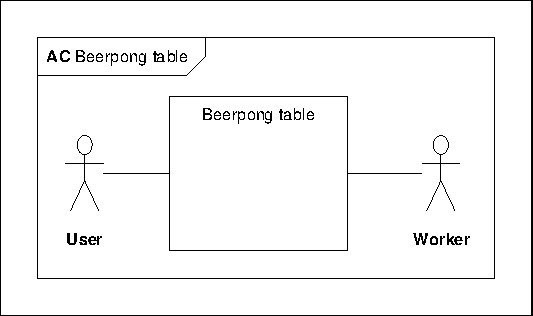
\includegraphics[width=0.8\textwidth,trim={0.24in 0.24in 0.24in 0.24in},clip, page=1]{Kravspecifikation/Graphics/Krav-spec-diagrammer.pdf}
    \caption{Aktør kontekst diagram for systemet}
    \label{fig:Actor-context}
\end{figure}

\subsection{Use Case Diagram}
Der benyttes use cases til at beskrive de funktionelle krav. Der er derfor lavet use case diagrammet som kan ses på figur \ref{fig:Use_case}.
\begin{figure}[!htb]
    \centering
    \includegraphics[width=0.8\textwidth,trim={0.24in 0.24in 0.24in 0.24in},clip, page=2]{Kravspecifikation/Graphics/Krav-spec-diagrammer.pdf}
    \caption{Use Case diagram for systemet}
    \label{fig:Use_case}
\end{figure}

\subsection{Use case beskrivelser (brief)}
\subsection{Use case beskrivelser (Fully dressed)}
\subsubsection{UC1: Start game}
\begin{table}[]
    \centering
    
\begin{tabular}[]{@{}ll@{}}
\hline
\hline

\begin{minipage}[t]{0.47\columnwidth}\raggedright
{Navn}\strut
\end{minipage} & \begin{minipage}[t]{0.47\columnwidth}\raggedright
{UC1 - Start spil}\strut
\end{minipage}\tabularnewline
\hline
\begin{minipage}[t]{0.47\columnwidth}\raggedright
{Mål}\strut
\end{minipage} & \begin{minipage}[t]{0.47\columnwidth}\raggedright
{The game is ready to be played}\strut
\end{minipage}\tabularnewline
\hline
\begin{minipage}[t]{0.47\columnwidth}\raggedright
{Initiering}\strut
\end{minipage} & \begin{minipage}[t]{0.47\columnwidth}\raggedright
{User}\strut
\end{minipage}\tabularnewline
\hline
\begin{minipage}[t]{0.47\columnwidth}\raggedright
{Aktører}\strut
\end{minipage} & \begin{minipage}[t]{0.47\columnwidth}\raggedright
{Primary: User}\strut
\end{minipage}\tabularnewline
\hline
\begin{minipage}[t]{0.47\columnwidth}\raggedright
{Referencer}\strut
\end{minipage} & \begin{minipage}[t]{0.47\columnwidth}\raggedright
{}\strut
\end{minipage}\tabularnewline
\hline
\begin{minipage}[t]{0.47\columnwidth}\raggedright
{Antal samtidige forekomster}\strut
\end{minipage} & \begin{minipage}[t]{0.47\columnwidth}\raggedright
{1}\strut
\end{minipage}\tabularnewline
\hline
\begin{minipage}[t]{0.47\columnwidth}\raggedright
{Prækondition}\strut
\end{minipage} & \begin{minipage}[t]{0.47\columnwidth}\raggedright
{The table has ping pong balls and is fully operational}\strut
\end{minipage}\tabularnewline
\hline
\begin{minipage}[t]{0.47\columnwidth}\raggedright
{Postkondition}\strut
\end{minipage} & \begin{minipage}[t]{0.47\columnwidth}\raggedright
{The table has dispensed 1 ping pong ball, the players have been setup in the system... og spillet er igang}\strut
\end{minipage}\tabularnewline
\hline
\begin{minipage}[t]{0.47\columnwidth}\raggedright
{Hovedscenarie}\strut
\end{minipage} & \begin{minipage}[t]{0.47\columnwidth}\raggedright
\begin{enumerate}
\tightlist
\item
  {The user places cups on the designated places on the table}
\item
  {The user inserts a coin into the coin slot}
\item
  {The table dispenses one ping pong ball, prepares the UI for
  player input and lights up LEDs around/underneath the cups}
\item
  {The player selects number of players on the UI}
\item
  {The player inputs team names on the UI}
\item
  {The player hits start on the UI}
\end{enumerate}\strut
\end{minipage}\tabularnewline
\hline
\begin{minipage}[t]{0.47\columnwidth}\raggedright
{Udvidelser eller undtagelser}\strut
\end{minipage} & \begin{minipage}[t]{0.47\columnwidth}\raggedright
{}\strut
\end{minipage}\tabularnewline
\hline
\begin{minipage}[t]{0.47\columnwidth}\raggedright
{Data variationsliste}\strut
\end{minipage} & \begin{minipage}[t]{0.47\columnwidth}\raggedright
{}\strut
\end{minipage}\tabularnewline
\hline
\hline
\end{tabular}
    \caption{Caption}
    \label{tab:UC1}
\end{table}



\end{document}
